\chapter{Numerical Ordinary Differential Equations}\label{ch:odes}
\begin{quote}
    {\it ``The mathematical discipline of differential equations furnishes the explanation of
    all those elementary manifestations of nature which involve time.''} \\
    --\href{https://en.wikipedia.org/wiki/Sophus_Lie#Legacy}{Norwegian
    Mathematician Sophus Lie}
\end{quote}

% In this chapter we will solve first order ordinary differential equations of the form
% \[ y'(t) = f(t,y(t)) \]
% with initial condition $y(t_0)=y_0$ for $t\ge t_0$.  These are known as ``ordinary''
% differential equations since they contain only ``ordinary'' derivatives; not partial
% derivatives.  Given that we are solving the problem with given initial information these
% are also called initial value problems.  


\section{Recalling the Basics of Ordinary Differential Equations}

\begin{problem}
    Sketch a plot of the function that would model each of the following scenarios.
    \begin{enumerate}
        \item[(a)] A population of an endangered species is slowly dying off.  The rate at
            which the population decreases is proportional to the amount of population
            that is presently there.  What does the population as a function of time look
            like for this species?
        \item[(b)] Consider a mass hanging from a spring that is suspended vertically from
            the ceiling.  If the mass is given an initial upward {\it bump} and then left
            alone, what will the position of the mass be as a function of time?
        \item[(c)] A pollutant has entered the tributary for a certain reservoir, and a
            small concentration leaks into the water over a long period of time.  The
            reservoir is dam controlled so the rate of release is well known and
            relatively constant.  What does the function modeling the amount of pollutant
            look like as time goes on?
        \item[(d)] A drug is eliminated from the body via natural metabolism.  Assume that
            there is some initial amount of drug in the body.  What does the function
            modeling the amount of drug in the system look like over time? 
    \end{enumerate}
\end{problem}

All of the functions that you played with in the previous problem can easily be modeled
with differential equations.  There are few tools in the mathematician's arsenal that are
more useful than modeling with differential equations.  We will focus the next two
chapters of the book on these types of equations and their numerical solutions, but first:
what is a differential equation?
\begin{definition}
    A {\bf differential equation} is an equation that relates the derivative (or
    derivatives) of an unknown function to itself.  
    \label{def:diff_eq}
\end{definition}

\begin{definition}
    A {\bf solution to a differential equation} is a function which, when substituted into
    the differential equation, creates a true statement.
    \label{def:soln_diff_eq}
\end{definition}

\begin{definition}
    A {\bf numerical solution to a differential equation} is a list of ordered pairs that
    gives a point-wise approximation to the actual solution.
    \label{def:num_soln_diff_eq}
\end{definition}
These ideas should be familiar to you from previous classes, but just in case, this
section gives a very brief review of some of the basics.

Solving differential equations analytically is a subject unto itself, but it is worth our
time here to revisit some of the basic techniques for solving differential equations.  It
should be noted that if an analytic solution exits then there is no reason to do any of
the numerical techniques that we will discuss in this chapter -- you're done if you have
an analytic solution.  The fact of the matter is, however, that the techniques for finding
analytic solutions to differential equations are rather limiting, and when the
differential equations get complicated we will only have numerical approximations to lean
back on.

Let's get started with some review.
\begin{problem}
    Identify which of the following problems are {\it differential} equations and which
    are {\it algebraic} equations.
    \begin{flalign*}
        x^2 + 5x &= 7x^3 - 2 \\
        x'' + 5x &= 7x''' - 2 \\
        y' + 5 &= -3y \\
        y''y'y &= 8 \\
        y^2 \cdot y &= 8 
    \end{flalign*}
    (Do not try to solve any of these equations)
\end{problem}

\begin{problem}
    Consider the differential equation $y' = 3y$ with an initial condition $y(0) = 4$.
    Which of the following functions is a solution to this differential equation, and what
    is the value of the constant in the function?
    \begin{enumerate}
        \item[(a)] $y(t) = C \sin(3 t)$
        \item[(b)] $y(t) = C e^{3t}$
        \item[(c)] $y(t) = C t^3$
        \item[(d)] $y(t) = t^3 + C$
        \item[(e)] $y(t) = e^{3t} + C$
        \item[(f)] $y(t) = \sin(3t) + C$
    \end{enumerate}
\end{problem}

\begin{problem}
    Consider the differential equation $y' = 3y + t$ with an initial condition $y(0) = 4$.
    Which of the following functions is a solution to this differential equation, and what
    are the values of the constants?
    \begin{enumerate}
        \item[(a)] $y(t) = C_0 \sin(\sqrt{3} t) + C_1 t + C_2$
        \item[(b)] $y(t) = C_0 e^{3t} + C_1 t + C_2$
        \item[(c)] $y(t) = C_0 t^3 + C_1 t + C_2$
        \item[(d)] $y(t) = C_3 t^3 + C_2 t^2 + C_1 t + C_0$
        \item[(e)] $y(t) = e^{3t} + C_1 t + C_2$
        \item[(f)] $y(t) = \sin(3t) + C_1 t + C_2$
    \end{enumerate}
\end{problem}

\begin{problem}
    Prove that the function $x(t) = -\frac{1}{2} \cos(2t) + \frac{7}{2}$ solves the
    differential equation $x' = \sin(2t)$ with the initial condition $x(0) =3$.
\end{problem}

\begin{technique}[Separation of Variables]
    To solve a differential equation of the form
    \[ \frac{dy}{dt} = f(y) g(t) \]
    we can separate the variables and rewrite the problem as 
    \[ \int \frac{dy}{f(y)} = \int g(t) dt. \]
    Integrating both sides and solving for $y(t)$ gives the solution.
\end{technique}

\begin{problem}
    Use separation of variables to solve the differential equation 
    \[ \frac{dy}{dt} = y\sin(t) \]
    with the initial condition $y(0) = 1$.
\end{problem}

\begin{problem}
    Solve the differential equation $y' = -2y + 12$ with $y(0) = 2$ using separation of
    variables. 
\end{problem}

\begin{problem}
    Consider the differential equation
    \[ \frac{dy}{dt} = -\frac{1}{4} y + 4 \]
    with the initial condition $y(0) = 7$.  
    \begin{enumerate}
        \item[(a)] Solve the differential equation using separation of variables.
        \item[(b)] Substitute your solution into the differential equation and verify that
            you are indeed correct in your work in part (a).
    \end{enumerate}
\end{problem}

There are MANY other techniques for solving differential equations, but a full discussion
of all of those techniques is beyond the scope of this book.  For the remainder of this
chapter we will focus on finding {\it approximate} solutions to differential equations.
It will be handy, however, to be able to check our work on problems where an analytic
solution is available.

\newpage\section{Euler's Method}

\begin{problem}\label{prob:euler_motivation}
    Consider the differential equation $y' = -0.5y$ with the initial condition $y(0) = 6$.  
    \begin{enumerate}
        \item[(a)] Since we know that $y(0) = 6$ and we know that $y'(0) = -0.5 \cdot y(0)$
            we can approximate the value of $y$ at some future time step.  Let's go 1 unit
            forward in time.  That is, approximate $y(1)$ knowing that $y(0) = 6$ and
            $y'(0) = -3$. \\
            Hint: We know a $y$-value, a slope, and the size of the step that we would
            like to move in the $t$ direction \ldots
            \[ y(1) \approx \underline{\hspace{1in}} \]
        \item[(b)] Use your answer from part (a) for time $t=1$ to approximate the $y$
            value at time $t=2$.  Then use that value to approximate the value at time
            $t=3$.  Repeat the process to approximate the value of $y$ at
            times $t=2, 3, 4, 5, \ldots, 10$.  Record your answers in the table below.
            Then find the analytic solution to this differential equation and record the
            $y$ values at the appropriate times.
            \begin{center}
                \begin{tabular}{|c|c|c|c|c|c|c|c|c|c|c|c|}
                    \hline
                    $t$ & 0 & 1 & 2 & 3 & 4 & 5 & 6 & 7 & 8 & 9 & 10 \\ \hline
                    Approximation of $y$ & 6 &   &   &   &   &   &   &   &   &   &   \\ \hline
                    Exact value of $y$ & 6 &   &   &   &   &   &   &   &   &   &   \\ \hline
                \end{tabular}
            \end{center}
        \item[(c)] The ``approximations of $y$'' that you found in part (b) are a {\bf
            numerical approximation} of the solution to the differential equation.  You
            should notice that your numerical solution is pretty far off from the actual
            solution for most values of $t$.  Why?  What could be the sources of this
            error and how could we fix it?  Once you have an idea of how to fix it, put
            your idea into action and devise some measurement of error to analyze your
            results.
        \item[(d)] Draw a clear picture of what this method is doing in order to
            approximate the slope at each individual step.
    \end{enumerate}
\end{problem}

The notion of approximating solutions to differential equations is simple: make a discrete
approximation to the derivative and step forward through time as a difference equation.
The fun part is making the approximation to the derivative(s).  There are many methods for
approximating derivatives, and that is exactly where we'll start.

\begin{technique}[Euler's Method]
    You're probably already familiar with Euler's method for approximating the solution to
    a differential equation. We want to approximate a solution to $y'(t) = f(t,y(t))$.
    Recall from Problem \ref{prob:num_diff_first_order} that 
    \[ y'(t) = \frac{y(t+h) - y(t)}{h} + \mathcal{O}(h) \]
    so the differential equation $y'(t) = f(y(t),t)$ becomes
    \[ \frac{y(t+h) - y(t)}{h} \approx f(y(t),t). \]
    Rewriting as a difference equation, letting $y_{n+1} = y(t_n+h)$ and $y_n = y(t_n)$,
    we get
    \begin{flalign}
        y_{n+1} = y_n + h f(y_n, t_n)
        \label{eqn:Eulers_method}
    \end{flalign}
%     \begin{enumerate}
%         \item Recall that a taylor series for a continuously differentiable function
%             $f(x)$ centered at $x=a$ is
%             \[ f(x) = f(c) + \frac{f'(a)}{1!}(x-a) + \frac{f''(a)}{2!}(x-a)^2 +
%                 \frac{f^{(3)}(a)}{3!}(x-a)^3 + \frac{f^{(4)}(a)}{4!}(x-a)^4 + \cdots \]
%         \item Write a Taylor series for $y(t)$ by replacing $f$ with $y$, $x$ with $t+h$
%             and $a$ with $t$
%             \[ y(t+h) = \dots\]
% %             \teacher{
% %                 \[ y(t+h) = y(t) + y'(t)h + \frac{y''(t)}{2!} h^2 + \cdots \]
% %             }
%         \item Since we know that $y'(t) = f(t,y(t))$ we can rewrite the Taylor series as
%             \[ y(t+h) = \dots \]
% %             \teacher{
% %                 \[ y(t+h) = y(t) + hf(t,y(t)) + \frac{y''(t)}{2!} h^2 + \cdots \]
% %             }
%         \item Now we can look at this as a difference equation that is ready made for
%             numerical implementation with a loop:
%             \[ y_{n+1} = y_n + h f(t_n,y_n) + \mathcal{O}(h^2)\]
%         \item The {\it approximation error} for Euler's method is actually not second
%             order as the previous equation would suggest.  Instead, if we rearrange to
%             write Euler's formula as an approximation of the derivative we get
%             \[ \frac{y_{n+1}-y_n}{h} = f(t_n,y_n) + \mathcal{O}(h). \]
%             What does this formula tell you about the accuracy of Euler's method?
%     \end{enumerate}
\end{technique}

A way to think about Euler's method is that at a given point, the slope is approximated by
the value of the right-hand side of the differential equation and then we step forward $h$
units in time following that slope.  Figure \ref{fig:Euler} shows a depiction of the idea.
Notice in the figure that in regions of high curvature Euler's method will overshoot the
exact solution to the differential equation.  However, taking $h \to 0$ theoretically
gives the exact solution at the tradeoff of needing infinite computational resources.

\begin{figure}[ht!]
    \begin{center}
        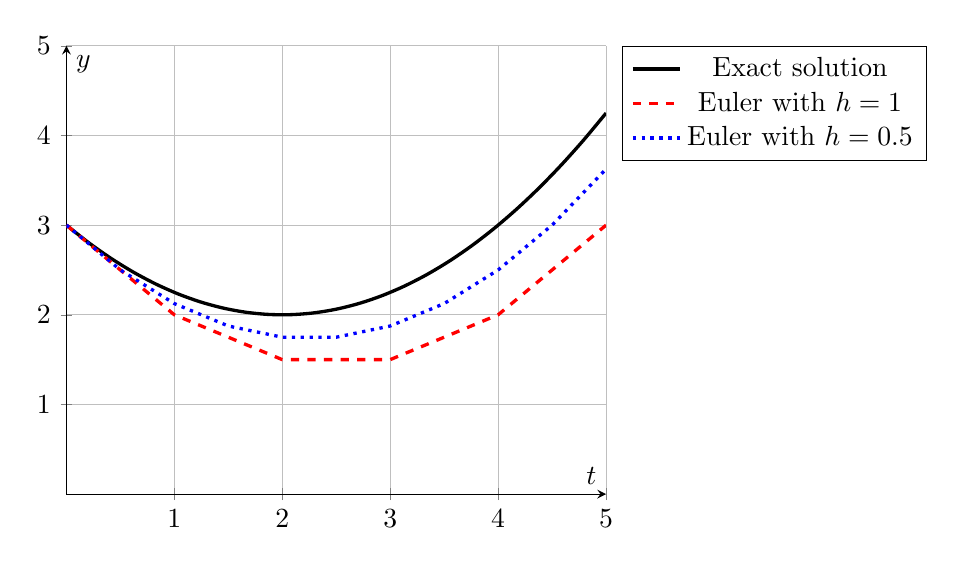
\begin{tikzpicture}
            \begin{axis}[axis lines=center, grid, xmin=0, xmax=5, ymin=0, ymax=5,
                domain=0:5, xlabel={$t$}, ylabel={$y$}, legend pos=outer north east]
                \addplot[very thick, smooth, black] {0.25*(x-2)^2+2};
                \addlegendentry{Exact solution};
                \addplot[red, dashed, very thick]
                coordinates{(0,3)(1,2)(2,1.5)(3,1.5)(4,2)(5,3)};
                \addlegendentry{Euler with $h=1$};
                \addplot[blue, dotted, very thick]
                coordinates{(0,3)(0.5,2.5)(1,2.125)(1.5,1.875)(2,1.75)(2.5,1.75)(3,1.875)(3.5,2.125)(4,2.5)(4.5,3)(5,3.625)};
                \addlegendentry{Euler with $h=0.5$};
            \end{axis}
        \end{tikzpicture}
    \end{center}
    \caption{A depiction of Euler's method with step size $h=1$ (red) and $h=0.5$ (blue).}
    \label{fig:Euler}
\end{figure}


\begin{problem}
    Write code to implement Euler's method for initial value problems.  Your \ProgLang
    function should accept as input: $f(y,t)$, \mcode{tmin}, \mcode{tmax}, the number of
    grid points (the value of $h = \Delta t$ should be calculated within your code), and
    an initial condition.  The output should be vectors for $t$ and $y$.\\
    \ifnum\Python=0
    \mcode{function [t,y] = MyEuler1D(f,tmin,tmax,num_pts,IC)} \\
    \else
    \mcode{def MyEuler1D(f,tmin,tmax,num_pts,IC):} \\
    \fi
    Test your code on a first order differential equation where you know the answer and
    then test your code on the differential equation
    \[ y' = -\frac{1}{3}y+\sin(t) \quad \text{where} \quad y(0) = 1. \]
\end{problem}


\begin{problem}\label{prob:ode_error_analysis}
    The differential equation $y' = -\frac{1}{3}y + \sin(t)$ with $y(0) = 1$ has an
    analytic solution 
    \[ y(t) = \frac{1}{10} \left( 19 e^{-t/3} + 3\sin(t) - 9\cos(t) \right). \]
    The goal of this problem will be to compare the maximum error on the interval $t \in
    [0,5]$ for various values of $\Delta t$ in your Euler solver.
    \begin{enumerate}
        \item[(a)] Write code that gives the maximum point-wise error between your
            numerical solution and the analytic solution given a value of $\Delta t$.
        \item[(b)] Using your code from part (a), build a plot with the value of $\Delta
            t$ on the horizontal axis and the value of the associated error on the
            vertical axis.  You should use a log-log plot.  Obviously you will need to run
            your code many times at many different values of $\Delta t$ to build your data
            set.
        \item[(c)] In general, if you were to cut your value of $\Delta t$ in half, what
            would that do to the value of the error?  What about dividing $\Delta t$ by
            10?  100?  1000?
    \end{enumerate}
\end{problem}


We can solve differential equations with multiple unknowns.  For example: the populations
of two competing species modeled over time.  These problems are typically very challenging
to solve by hand, but numerically the idea is exactly the same as with one-dimensional
Euler's method.  The problem is to simultaneously solve the equations
\begin{flalign*}
    x' = f(x,y,t) \\ 
    y' = g(x,y,t)
\end{flalign*}
where $x(t)$ and $y(t)$ are the functions we want to know, and $f$ and $g$ are functions
that model the system of interest.  Consider the following example of a system of
differential equations
\begin{flalign*}
    x' &= 0.5 xy - y \\ 
    y' &= 2y - 0.1xy^2 - t.
\end{flalign*}
In this example, $f(x,y,t) = 0.5xy - y$ and $g(x,y,t) = 2y - 0.1xy^2 - t$.  The changes in
the functions $x(t)$ and $y(t)$ are coupled together -- as one changes then so must the
other.  While this system of equations
might be impossible to solve analytically, we can approximate both of the derivatives in
the same way that we did with Euler's method in 1D and get a reasonable way to step this
differential equation forward in time.  Indeed,
\begin{flalign*}
    x' \approx \frac{x_{n+1} - x_n}{\Delta t} &= 0.5 x_n y_n - y_n \\ 
    y' \approx \frac{y_{n+1} - y_n}{\Delta t} &= 2 y_n - 0.1 x_n y_n^2 - t_n.
\end{flalign*}
After simplifying a bit we get
\begin{flalign*}
    x_{n+1} &= x_n + \Delta t \left( 0.5 x_n y_n - y_n \right) \\ 
    y_{n+1} &= y_n + \Delta t \left( 2 y_n - 0.1 x_n y_n^2 - t_n \right).
\end{flalign*}
As you can see, this is now a system of difference equations that can be coded with
relative ease.

\begin{technique}[2D Euler's Method]
    If 
    \begin{flalign*}
        x' &= f(x,y,t) \\
        y' &= g(x,y,t)
    \end{flalign*}
    then we can build a system of difference equations to approximate the solution by
    taking a first-order approximation of the derivatives and rewriting the system as 
    \begin{flalign*}
        x_{n+1} &= x_n + \underline{\hspace{1in}} \\
        y_{n+1} &= y_n + \underline{\hspace{1in}}.
    \end{flalign*}
\end{technique}


\begin{problem}
    Write a \ProgLang function for 2D Euler's method.  Test your code on a problem where you
    know the qualitative solution and can easily graphically check the answer.
\end{problem}


\begin{problem}\label{prob:2dPredPrey}
    Test your code from the previous problem on the
    following by showing a time evolution plot (time on $x$ and populations on
    $y$) as well as a phase plot ($x$ on the $x$ and $y$ on the $y$ with time understood
    implicitly):\\
    {\bf The Lotka-Volterra Predator-Prey Model:}\\
    Let $x(t)$ denote the number of rabbits (prey) and $y(t)$ denote the number of foxes
    (predator) at time $t$.  The relationship between the species can be modeled by the
    classic 1920's Lotka-Volterra Model:
    \[ \left\{ \begin{array}{ll} x' &= \alpha x - \beta xy \\ y' &= -\delta y + \gamma xy
        \end{array} \right. \]
    where $\alpha, \beta, \gamma,$ and $\delta$ are positive constants.  For this
    problems take $\alpha \approx 1$, $\beta \approx 0.05$, $\gamma \approx 0.01$, and
    $\delta \approx 1$.  Be sure to explain the meaning of each of the parameters and each
    of the components of the model.
\end{problem}



\newpage\section{The Midpoint Method}

\begin{problem}
    Let's return to the simple differential equation $y' = -0.5y$ with $y(0) = 6$ that we
    saw in Problem \ref{prob:euler_motivation}.  Now we'll propose a slightly different
    method for approximating the solution.
    \begin{enumerate}
        \item[(a)] At $t=0$ we know that $y(0)=6$.  If we use the slope at time $t=0$ to
            step forward in time then we will get the Euler approximation of the solution.
            Consider this alternative approach: 
            \begin{itemize}
                \item Use the slope at time $t=0$ and move {\it half} a step forward.  
                \item Find the slope at the half-way point
                \item Then use the slope from the half way point to go a full step forward
                    from time $t=0$.  
            \end{itemize} 
            Perhaps a bit confusing \ldots let's build this idea together:
            \begin{itemize}
                \item What is the slope at time $t=0$? $y'(0) =
                    \underline{\hspace{0.5in}}$
                \item Use this slope to step a half step forward and find the $y$ value:
                    $y(0.5) \approx \underline{\hspace{0.5in}}$
                \item Now use the differential equation to find the slope at time $t=0.5$.
                    $y'(0.5) = \underline{\hspace{0.5in}}$
                \item Now take your answer from the previous step, and go one full step
                    forward from time $t=0$.  What $y$ value do you end up with? 
                \item Your answers to the previous bullets should be: $y'(0) = -3$, $y(0.5) \approx
                    4.5$, $y'(0.5) = -2.25$, so if we take a full step forward with slope
                    $m=-2.25$ starting from $t=0$ we get $y(1) \approx 3.75$.
            \end{itemize}
        \item[(b)] Repeat the process outlines in part (a) to approximate the solution to
            the differential equation at times $t=2, 3, \ldots, 10$.  Also record the
            exact answer at each of these times.
            \begin{center}
                \begin{tabular}{|c|c|c|c|c|c|c|c|c|c|c|c|}
                    \hline
                    $t$ & 0 & 1 & 2 & 3 & 4 & 5 & 6 & 7 & 8 & 9 & 10 \\ \hline
                    Approximation of $y$ & 6 &   &   &   &   &   &   &   &   &   &   \\ \hline
                    Exact value of $y$ & 6 &   &   &   &   &   &   &   &   &   &   \\ \hline
                \end{tabular}
            \end{center}
        \item[(c)] Draw a clear picture of what this method is doing in order to
            approximate the slope at each individual step.
        \item[(d)] How does your approximation compare to the Euler approximation that you
            found in Problem \ref{prob:euler_motivation}? 
    \end{enumerate}
\end{problem}

\begin{technique}[The Midpoint Method]
    Now we begin the journey of creating better solvers than Euler's method.  The midpoint method
    is defined by first taking a half step with Euler's method to approximate a solution
    at time $t_{n+1/2} \equiv (t_n + t_{n+1})/2$ and then taking a full step using the
    value of $f$ at $t_{n+1/2}$ and the approximate $y_{n+1/2}$.
    \begin{flalign*}
        y_{n+1/2} &= y_n + \frac{h}{2} f(y_n, t_n) \\
        y_{n+1} &= y_n + h f(y_{n+1/2}, t_{n+1/2})
    \end{flalign*}
    Note: Indexing by $1/2$ in a computer is nonsense.  Instead, we implement the midpoint
    method with:
    \begin{flalign*}
        y_{temp} &= y_n + \frac{h}{2} f(y_n, t_n) \\
        y_{n+1} &= y_n + h f\left( y_{temp}, \frac{t_n+t_{n+1}}{2}\right)
    \end{flalign*}

\end{technique}

\begin{problem}
    Write \ProgLang code to implement the midpoint method\\
    \ifnum\Python=1
    \mcode{function [t,y]=MyMidpointMethod(f,tmin,tmax,num_pts,IC)} \\
    \else
    \mcode{def MyMidpointMethod(f,tmin,tmax,num_pts,IC):} \\
    \fi
\end{problem}

\begin{problem}
    Repeat Problem \ref{prob:ode_error_analysis} with the midpoint method.  Compare your
    results to what you found with Euler's method.
\end{problem}

\begin{problem}
    Test your midpoint method code against your Euler1D code on the same single variable
    ODE as before.  You will likely see very little difference on a very small step size
    (equivalently, a large number of points), but for a smaller number of points there
    will be a remarkable difference.  
\end{problem}

We have studied two methods thus far: Euler's method and the Midpoint method.  In Figure
\ref{fig:Euler_Midpoint} we see a graphical depiction of how each method works on the
differential equation $y' = y$ with $\Delta t = 1$ and $y(0) = 1$.  The exact solution
at $t=1$ is $y(1) = e^1 \approx 2.718$ and is shown in red in each figure.  The methods
can be summarized as 
\begin{center}
    \begin{tabular}{|l|l|}
        \hline
        Euler's Method & Midpoint Method \\ \hline \hline
        1. Get the slope at time $t_n$ & 1. Get the slope at time $t_n$ \\ \hline
        2. Follow the slope for time $\Delta t$ & 2. Follow the slope for time $\Delta
        t/2$ \\ \hline
        & 3. Get the slope at the point $t_n  + \Delta t/2$ \\ \hline
        & 4. Follow the new slope from time $t_n$ for time $\Delta t$ \\ \hline
    \end{tabular}
\end{center}

\begin{figure}[ht!]
    \begin{center}
        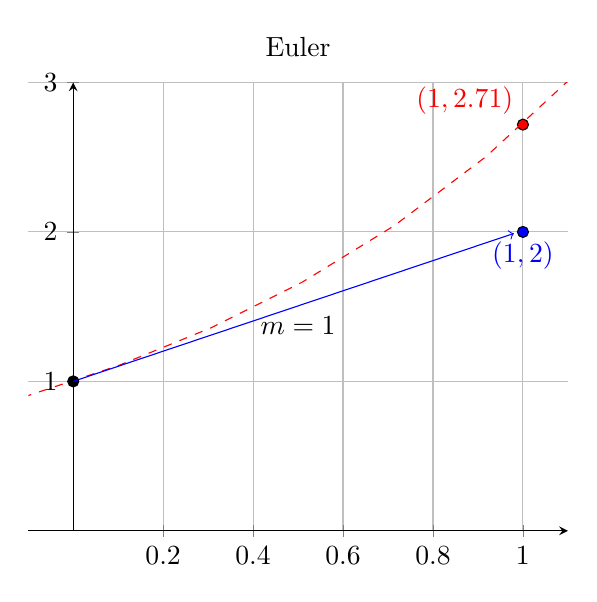
\begin{tikzpicture}
            \begin{axis}[axis lines=center, grid, xmin=-0.1, xmax=1.1, ymin=0, ymax=3,
                title={Euler}]
                \draw[fill=red] (axis cs:1,2.7182) circle(0.07cm); 
                \addplot[dashed, red, samples=50] {1*exp(x)};
                \draw[fill=black] (axis cs:0,1) circle(0.07cm); 
                \draw[blue, ->] (axis cs:0,1) -- (axis cs:0.98,1.99);
                \draw[fill=blue] (axis cs:1,2) circle(0.07cm);
                \draw (axis cs:0.5,1.5) node[anchor=north]{$m=1$};
                \draw[color=blue] (axis cs:1,2) node[anchor=north]{$(1,2)$};
                \draw[color=red] (axis cs:1,2.7182) node[anchor=south east]{$(1,2.71)$};
            \end{axis}
        \end{tikzpicture}
        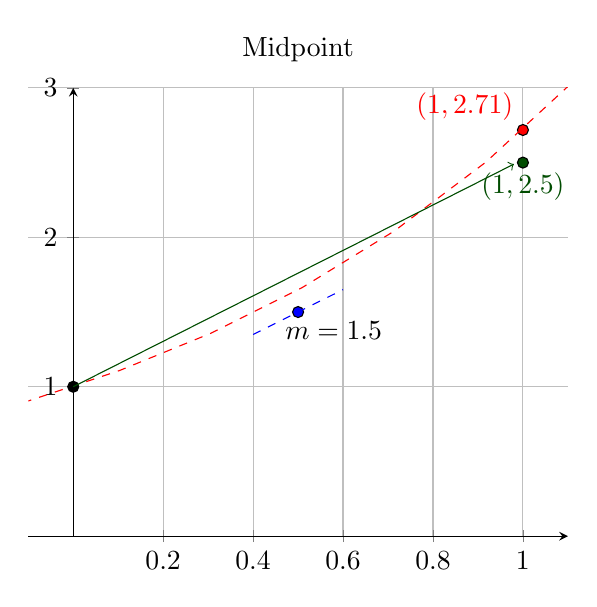
\begin{tikzpicture}
            \begin{axis}[axis lines=center, grid, xmin=-0.1, xmax=1.1, ymin=0, ymax=3,
                title={Midpoint}]
                \draw[fill=red] (axis cs:1,2.7182) circle(0.07cm); 
                \addplot[dashed, red, samples=50] {1*exp(x)};
                \draw[fill=black] (axis cs:0,1) circle(0.07cm); 
                \draw[fill=blue] (axis cs:0.5,1.5) circle(0.07cm);
                \draw[color=blue, dashed] (axis cs:0.4,1.35) -- (axis cs:0.6,1.65);
                \draw (axis cs:0.45,1.5) node[anchor=north west]{$m=1.5$};
                \draw[color=green!30!black, ->] (axis cs:0,1) -- (axis cs:0.98,2.49);
                \draw[fill=green!30!black] (axis cs:1,2.5) circle(0.07cm);
                \draw[color=green!30!black] (axis cs:1,2.5) node[anchor=north]{$(1,2.5)$};
                \draw[color=red] (axis cs:1,2.7182) node[anchor=south east]{$(1,2.71)$};
            \end{axis}
        \end{tikzpicture}
    \end{center}
    \caption{Graphical depictions of two numerical methods: Euler (left) and Midpoint
    (right). Here we use the simple differential equation
$y'=y$ with $y(0) = 0.5$ and $\Delta t = 1$.  The exact solution is shown in red.}
    \label{fig:Euler_Midpoint}
\end{figure}

\begin{problem}
    When might you want to use Euler's method instead of the midpoint method?  When might
    you want to use the midpoint method instead of Euler's method?
\end{problem}

\newpage\section{The Runge-Kutta Method}

\begin{problem}
    Again we return to the differential equation $y' = -0.5y$ with $y(0) = 6$ that we saw
    in Problem \ref{prob:euler_motivation}.  This time we'll walk through a slightly more
    challenging algorithm for approximating the slope solution to the differential
    equation.  In this algorithm we will make four approximations of the slope at a point
    and then use a weighted average of these four to take a full step forward.  The four
    approximations will be called $k_1, k_2, k_3$, and $k_4$.
    \begin{enumerate}
        \item[(a)] At $t=0$ we know that $y(0) = 6$.  Therefore, what is the slope at
            $t=0$?  $y'(0) = \underline{\hspace{0.5in}}$.  We will call this value $k_1$.
        \item[(b)] To calculate $k_2$ we take a half-step forward using the slope $k_1$.
            Using this slope, at time $t=0.5$ we find that $y'(0.5) =
            \underline{\hspace{0.5in}}$.  We will call this value $k_2$.
        \item[(c)] To calculate $k_3$ we take another half-step forward from the starting
            point but this time using the slope $k_2$.  Using this slope, at the $t = 0.5$
            we find that $y'(0.5) = \underline{\hspace{0.5in}}$.  We will call this value
            $k_3$.
        \item[(d)] To calculate $k_4$ we now take a full step forward using the slope
            $k_3$.  Using this slope we find that at $t=1$ we have $y'(1) =
            \underline{\hspace{0.5in}}$.  Call this slope $k_4$.
        \item[(e)] To check your work you should now verify that 
            \begin{flalign*}
                y(0) = 6 \quad \implies  y'(0) = -0.5 \cdot 6 = -3 \quad \implies 
                k_1 &= -3 \\
                y(0.5) \approx 6 - \frac{1}{2} \cdot 3 = 4.5 \quad \implies  y'(0.5) = -0.5 \cdot 4.5 = -2.25
                \quad \implies  k_2 &= -2.25 \\
                y(0.5) \approx 6 - \frac{1}{2} \cdot 2.25 = 4.875 \quad \implies 
                y'(0.5) = -0.5 \cdot 4.875 = -2.4375 \quad \implies  k_3 &= -2.4375 \\
                y(1) \approx 6 - 2.4375 = 3.5625 \quad \implies y'(1) = -0.5 \cdot 3.5625
                = -1.78125 \quad \implies k_4 &= -1.78125
            \end{flalign*}
            If your answers don't match then go back to parts (a) - (d) and check your
            thinking and arithmetic.
        \item[(f)]  We now have four approximations of the slope at the point $t=0$.  To
            move forward take a weighted average of these four approximations
            \[ \text{slope} \approx \frac{1 k_1 + 2 k_2 + 2 k_3 + 1k_4}{6}. \]
            Calculate this new slope and step forward one full step.  You should find that
            your approximate slope is $-2.359375$ and this gives an approximate value of
            $y(1)$ as $y(1) \approx 6 - -2.359375 = 3.640625$.  Compare this to the exact
            value of the solution to the differential equation at $t=1$.  You should see
            that you have some pretty amazing accuracy!!
        \item[(g)] Push this process forward one more step by hand.  Use the table below
            to summarize your results.
            \begin{center}
                \begin{tabular}{|c|c|c|c|}
                    \hline
                    $t$ & $0$ & $1$ & $2$ \\ \hline
                    $k_1$ & $-3$ & & $\times$ \\ \hline
                    $k_2$ & $-2.25$ & & $\times$ \\ \hline
                    $k_3$ & $-2.4375$ & & $\times$ \\ \hline
                    $k_4$ & $-1.78125$ & & $\times$ \\ \hline
                    Approximation of slope & $-2.359375$ & & $\times$ \\ \hline
                    Approximation of $y$ & $6$ & $3.640625$ & \\ \hline
                    Exact Value of $y$ & $6$ & $3.639184$ & \phantom{2.2072766} \\ \hline
                \end{tabular}
            \end{center}
    \end{enumerate}
\end{problem}

The method that you stepped through in the previous problem is called the Runge-Kutta 4
method for approximating the solution to an ordinary differential equation. It is one of a
family of many different approximation methods.  The ``4'' in the name is
not simply the fact that we are making four approximations of the slope, but in that it
enjoys fourth-order accuracy -- far better than both the Euler and Midpoint methods.
\begin{technique}[The Runge-Kutta 4 (RK4) Method]
    The Runge-Kutta 4 method is one (of many) such methods.  In this method, each $k_j$ is
    an approximation of the slope and we combine them in as a weighted average in the end.
    \begin{flalign*}
        k_1 &= f(y_n,\, t_n) \\
        k_2 &= f(y_n + \frac{h}{2} k_1,\, t_n + \frac{h}{2}) \\
        k_3 &= f(y_n + \frac{h}{2} k_2,\, t_n + \frac{h}{2}) \\
        k_4 &= f(y_n + h k_3,\, t_n + h) \\
        y_{n+1} &= y_n + \frac{h}{6} \left( k_1 + 2 k_2 + 2 k_3 + k_4 \right)
    \end{flalign*}
\end{technique}

Before we write code to implement the RK4 method we will examine it graphically just as we
did with Euler's method and the Midpoint method in Figure \ref{fig:Euler_Midpoint}.  For
simplicity we will examine the differential equation $y' = y$ with initial condition $y(0)
=1$ and $\Delta t = 1$.  In Figure \ref{fig:RK4_graphical} the red dashed line is the
exact solution $y(t) = e^t$.  In this example, $k_1 = 1$, $k_2 = 1.5$, $k_3 = 1.75$, and
$k_4 = 2.75$.  Hence the final slope propogating forward with $\Delta t = 1$ is 
\[ \frac{1}{6} \left(  1 + 2(1.5) + 2(1.75) + 2.75 \right) = 1.708. \]
Propogating this forward from the point $(0,1)$ gives the new point $(1,2.708)$.  Knowing
that $e \approx2.718$ we see a very high level of accuracy even with a really large time
step!

\begin{center}
    \begin{tabular}{|l|}
        \hline
        Runge-Kutta 4 Method \\ \hline \hline
        1. $k_1$ is the slope evaluated at time $t_n$ \\ 
        Project this slope half a step forward from time $t_n$ to the point $y_1$ \\ \hline
        2. $k_2$ is the slope evaluated at $y_1$ \\ 
        Project the slope $k_2$ half a step forward from time $t_n$ to the point $y_2$
        \\ \hline
        3. $k_3$ is the slope evaluated at the point $y_2$ \\
        Project the slope $k_3$ a full step foward from time $t_n$ to the point $y_3$ \\
        \hline
        4. $k_4$ is the slope evaluated at the point $y_3$ \\ \hline
        5. Project forward with slope $\frac{1}{6}(k_1 + 2k_2 + 2k_3 + k_4)$ from time
        $t_n$ \\ \hline
    \end{tabular}
\end{center}

\begin{figure}[ht!]
    \begin{center}
        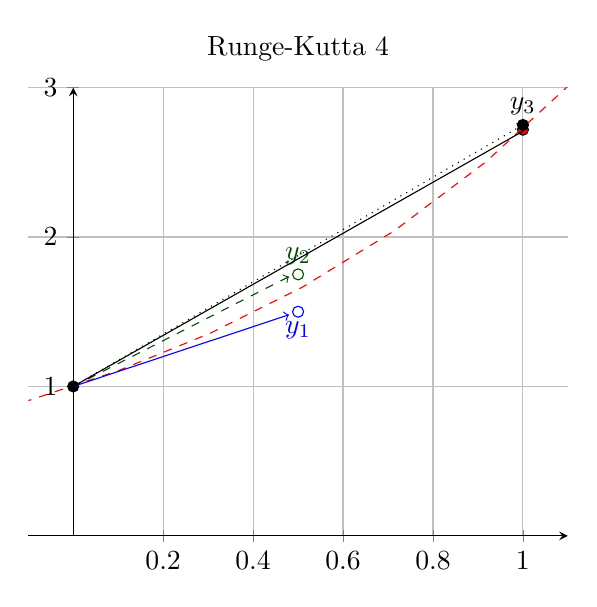
\begin{tikzpicture}
            \begin{axis}[axis lines=center, grid, xmin=-0.1, xmax=1.1, ymin=0, ymax=3,
                title={Runge-Kutta 4}]
                \draw[fill=red] (axis cs:1,2.7182) circle(0.07cm); 
                \addplot[dashed, red, samples=50] {1*exp(x)};
                \draw[fill=black] (axis cs:0,1) circle(0.07cm); 
                \draw[blue,->] (axis cs:0,1) -- (axis cs:0.48,1.48);
                \draw[blue] (axis cs:0.5,1.5) circle(0.07cm) node[anchor=north]{$y_1$};
%                 \draw (axis cs:0.05,1.1) node[anchor=north west]{$k_1 = 1$};
                \draw[color=green!30!black, dashed, ->] (axis cs:0,1) -- (axis
                cs:0.48,1.735);
                \draw[color=green!30!black] (axis cs:0.5,1.75) circle(0.07cm);
                \draw[color=green!30!black] (axis cs:0.5,1.75) node[anchor=south]{$y_2$};
                \draw[color=black, dotted, ->] (axis cs:0,1) -- (axis cs:1,2.75);
                \draw[fill=black] (axis cs:1,2.75) circle(0.07cm);
                \draw (axis cs:1,2.75) node[anchor=south]{$y_3$};
                \draw (axis cs:0,1) -- (axis cs:1,2.708);
            \end{axis}
        \end{tikzpicture}
    \end{center}
    \caption{Graphical depiction of the RK4 method.  The red dashed curve gives the exact
    solution to the differential equation $y' = y$ with initial condition $y(0) = 1$. The
solid black line gives the final projection.}
    \label{fig:RK4_graphical}
\end{figure}

\begin{problem}
    Write a \ProgLang function that implements the Runge-Kutta 4 method in one dimension.\\
    \ifnum\Python=0
    \mcode{function [t,y]=MyRk4(f,tmin,tmax,num\_pts,IC)} \\
    \else
    \mcode{def MyRk4(f,tmin,tmax,num\_pts,IC):} \\
    \fi
    Test the problem on a known differential equation.
\end{problem}


\begin{problem}
    Repeat Problem \ref{prob:ode_error_analysis} with the Runge Kutta method.  Compare your
    results to what you found with Euler's method and with the midpoint method.
\end{problem}


\begin{problem}
    Modify your Runge-Kutta 4 code to work for two dependent variables.  I'll get you
    started:\\We want to solve
    \[ \left\{ \begin{array}{ll} x' &= f(x,y,t) \\ y' &= g(x,y,t) \end{array} \right. \]
    and to do so we extend the Runge Kutta method as
    \begin{flalign*}
        k_1 &= f(x_n, y_n,t_n) \\
        q_1 &= g(x_n, y_n, t_n,) \\
        k_2 &= f(x_n+\frac{h}{2} k_1, y_n + \frac{h}{2} q_1, t_n + \frac{h}{2}) \\
        q_2 &= g(x_n+\frac{h}{2} k_1, y_n + \frac{h}{2} q_1,t_n + \frac{h}{2}) \\
        k_3 &= \dots \\
        q_3 &= \dots \\
        k_4 &= \dots \\
        q_4 &= \dots \\
        x_{n+1} &= x_n + \frac{h}{6} \left( k_1 + 2 k_2 + 2 k_3 + k_4 \right)\\
        y_{n+1} &= y_n + \frac{h}{6} \left( q_1 + 2 q_2 + 2 q_3 + q_4 \right)
    \end{flalign*}
    
    Test your code on
    the predator prey model in problem \ref{prob:2dPredPrey}.
\end{problem}


\begin{problem}
    Solving \underline{systems} of ordinary differential equations would become challenging if we were
    to continue coding in the same way as in the previous problem -- modifying your code
    to account for the number of differential equations. Write a \ProgLang function
    that accepts any number of right-hand sides from a system of differential equations
    and then leverages the fact that \ProgLang works very well with vectors to create Euler
    and Runge-Kutta solutions to these systems. Devise several systems to test your code
    (including 1D and 2D).

    One particular nonlinear system of differential equations that you can test on is
    \[ \left\{ \begin{array}{rlc} y_1' &= -0.1y_2 y_1 - y_1 & y_1(0) = 2 \\
            y_2' &= -y_1 + 0.9y_2 & y_2(0) = 1 \\
        y_3' &= \sin(t)+ \cos(y_2) & y_3(0)=-2 \end{array} \right.. \]
    Note that we would probably never try to solve this problem by hand so a numerical
    method is warranted.

    A test script to check your General Euler and General RK code is as follows.  You can
    use my notation here to possibly reverse engineer the construction of your general ODE
    solver codes.

    \bcode
\begin{lstlisting}
numpts = 1000;
f = @(t,y) [-0.1*y(2)*y(1)-y(1) ; 
    -y(1)+0.9*y(2) ; 
    sin(t) + cos(y(2))];

tmax = 5.5;

[t,yeuler]=MyGeneralEuler(f,0,tmax,numpts,[2,1,-2]);
plot(t,yeuler(1,:),'b--',t,yeuler(2,:),'r--',t,yeuler(3,:),'k--')
hold on

[t,yrk]=MyGeneralRK4(f,0,tmax,numpts,[2,1,-2]);
plot(t,yrk(1,:),'k-.',t,yrk(2,:),'m-.',t,yrk(3,:),'c--')
grid on
legend('y_1''(t)' , 'y_2''(t)' , 'y_3''(t)')
\end{lstlisting}
    \ifnum\Python=1
{\color{red} Note: Build some sample code for this problem in the Python version}
\fi
\end{problem}




\newpage\section{The Backwards Euler Method}
\begin{problem}
    The major trouble with the RK (and midpoint) methods is that they take many more
    function evaluations than Euler's method.  We can improve upon Euler's method in the
    following way:\\
    We want to solve $y' = f(t,y)$ so:
    \begin{enumerate}
        \item Approximate the derivative by looking forward in time(!)
            \[ \frac{y_{n+1} - y_n}{h} \approx f(y_{n+1}, t_{n+1}) \]
        \item Rearrange to get the difference equation
            \[ y_{n+1} = y_n + h f(y_{n+1},t_{n+1}). \]
        \item Notice that we \underline{will} have $t_{n+1}$ but we \underline{do not
            have} $y_{n+1}$.  The major trouble is that $y_{n+1}$ shows up on both sides
            of the equation.  Can you think of a way to solve for it? \dots you have code
            that does this step!!!
        \item This method is called the {\bf backward Euler} method and is known as an
            {\bf implicit method} since you need to solve a nonlinear equation at each
            step.  The advantage (usually) is that you can take far fewer steps with
            reasonably little loss of accuracy.
    \end{enumerate}
\end{problem}

\begin{problem}
    Let's take a few steps through the backward Euler method on a problem that we know
    well: $y' = -0.5y$ with $y(0) = 6$.  \\
    Let's take $h=1$ for simplicity, so the backward Euler iteration scheme for this
    particular differential equation is
    \[ y_{n+1} = y_n - \frac{1}{2} y_{n+1}. \]
    Notice that $y_{n+1}$ shows up on both sides of the equation.  A little bit of
    rearranging gives 
    \[ \frac{3}{2} y_{n+1} = y_n \quad \implies \quad y_{n+1} = \frac{2}{3} y_n. \]
    \begin{enumerate}
        \item[(a)] Complete the following table.
            \begin{center}
                \begin{tabular}{|c|c|c|c|c|c|c|c|c|c|c|c|}
                    \hline
                    $t$ & 0 & 1 & 2 & 3 & 4 & 5 & 6 & 7 & 8 & 9 & 10 \\ \hline
                    Euler Approx. of $y$ & 6 & 3  & 1.5  & 0.75  &   &   &   &   &   &   &   \\ \hline
                    Back. Euler Approx.of $y$ & 6 & 4  & 2.667  & 1.778  &   &   &   &   &   &   &   \\ \hline
                    Exact value of $y$ & 6 & 3.64  & 2.207  & 1.339  &   &   &   &   &   &   &   \\ \hline
                \end{tabular}
            \end{center}
        \item[(b)] Compare now to what we found for the midpoint method on this problem as
            well.
    \end{enumerate}
\end{problem}

\begin{problem}
    The previous problem could potentially lead you to believe that the backward Euler
    method will always result in some other nice difference equation.  That isn't true!
    Let's consider a slightly more complicated differential equation and see what happens
    \[ y' = -\frac{1}{2} y^2 \quad \text{with} \quad y(0) = 0. \]
    \begin{enumerate}
        \item[(a)] Recall that the backward Euler approximation is 
            \[ y_{n+1} = y_n + h f(y_{n+1},t_{n+1}). \]
            Let's take $h=1$ for simplicity (we'll make it smaller later).  What is the
            backward Euler formula for this particular differential equation?
        \item[(b)] You should notice that your backward Euler formula is now a quadratic
            function in $y_{n+1}$.  That is to say, if you are given a value of $y_n$ then
            you need to solve a quadratic polynomial equation to get $y_{n+1}$.  Let's be
            more explicit: \\
            We know that $y(0) = 6$ so in our numerical solutions, $y_1 = 6$.  In order to
            get $y_2$ we consider the equation $y_2 = y_1 - \frac{1}{2} y_2^2$.
            Rearranging we see that we need to solve $\frac{1}{2}y_2^2 + y_2 - 6 = 0$
            in order to get $y_2$.  Doing so gives us $y_2 = \sqrt{13} - 1 \approx 2.606$.
        \item[(c)] Go two steps further with the backward Euler method on this problem.
            Then take the same number of steps with regular (forward) Euler's method.
        \item[(d)] Work our the analytic solution for this differential equation (using
            separation of variables perhaps).  Then compare the values that you found in
            parts (b) and (c) of this problem to values of the analytic solution and
            values that you would find form the regular (forward) Euler approximation.
    \end{enumerate}
\end{problem}

The complications with the backward Euler's method are that you have a nonlinear equation
to solve at every time step
\[ y_{n+1} = y_n + h f(y_{n+1},t_{n+1}). \]
Notice that this is the same as solving the equation
\[ y_{n+1} - hf(y_{n+1},t_{n+1}) - y_n = 0. \]
You know the values of $h$, $t_{n+1}$ and $y_n$, and you know the function $f$, so, in a practical sense, you should use some sort of Newton's
method iteration to solve that equation -- at each time step.  One seed for your Newton's method could be the
value from the previous time step since you likely don't expect your solution to change
wildly from step to step.  Following this logic, if you expect a solution at least {\it
close} to where you currently are, then only a few steps of Newton's method should suffice
(perhaps only 5 or 10!).  You may want to experiment with how many steps of Newton's
method you need to solve and still maintain some accuracy in your method.


\begin{problem}
    Write \ProgLang code to implement the backward Euler's method for a 1D initial value
    problem. \\
    \ifnum\Python=0
    \mcode{function [t,y] = MyBackwardEuler(f, tmin, tmax, num_pts, IC)}
    \else
    \mcode{def MyBackwardEuler(f, tmin, tmax, num_pts, IC):}
    \fi
\end{problem}


\begin{problem}
    Write a \ProgLang script that outputs a log-log plot with the step size on the horizontal
    axis and the error in the numerical method on the vertical axis.  Plot the errors for
    Euler, Midpoint, Runge Kutta, and Backward Euler measured against a differential
    equation with a known analytic solution.  Use this plot to conjecture the convergence
    rates of the four methods.
\end{problem}



\newpage\section{Exercises}

\subsection{Algorithm Summaries}

\begin{problem}
    Consider the first-order differential equation $y' = f(y,t)$.  What is Euler's method
    for approximating the solution to this differential equation?  What is the order of
    accuracy of Euler's method?  Explain the meaning of the order of the method in the
    context of solving a differential equation.
\end{problem}

\begin{problem}
    Explain in clear language what Euler's method does geometrically.
\end{problem}

\begin{problem}
    Consider the first-order differential equation $y' = f(y,t)$.  What is the Midpoint method
    for approximating the solution to this differential equation?  What is the order of
    accuracy of the Midpoint method?  Explain the meaning of the order of the method in the
    context of solving a differential equation.
\end{problem}
\begin{problem}
    Explain in clear language what the Midpoint method does geometrically.
\end{problem}

\begin{problem}
    Consider the first-order differential equation $y' = f(y,t)$.  What is the Runge Kutta
    method for approximating the solution to this differential equation?  What is the
    order of accuracy of the Runge Kutta method?  Explain the meaning of the order of the
    method in the context of solving a differential equation.
\end{problem}

\begin{problem}
    Explain in clear language what the Runge Kutta method does geometrically.
\end{problem}

\subsection{Applying What You've Learned}
\begin{problem}
    Test the Euler, Midpoint, and Runge Kutta methods on the differential
    equation
    \[ y' = \lambda \left( y - \cos(t) \right) - \sin(t) \quad \text{with} \quad y(0) = 1.5. \]
    Find the exact solution by hand using the method of undetermined coefficients and note
    that your exact solution will involve the parameter $\lambda$.  Produce log-log plots
    for the error between your numerical solution and the exact solution for $\lambda =
    -1$, $\lambda = -10$, $\lambda = -10^2$, \ldots, $\lambda = -10^6$.  In other words,
    create 7 plots (one for each $\lambda$) showing how each of the 3 methods performs for
    that value of $\lambda$ at different values for $\Delta t$.
\end{problem}
\hint{
    Let the maximum time be small and take a large number of time steps.
}


\begin{problem}
    We wish to solve the boundary valued problem $x'' + 4x = \sin(t)$ with initial
    condition $x(0)=1$ and boundary condition $x(1)=2$.  Notice that you do not have the
    initial position and initial velocity as you normally would with a second order
    differential equation.  Devise a method for finding a numerical solution to this
    problem. \\
    Hint: First write the problem as a system of first order differential equations.  Then
    think about how your bisection method code might help you.
\end{problem}


\begin{problem}
    Write code to solve the boundary valued differential equation
    \[ y'' = \cos(t) y' + \sin(t) y \quad \text{with} \quad y(0) = 0 \quad \text{and}
        \quad y(1) = 1. \]
\end{problem}
\hint{
    Introduce an auxiliary variable $v = y'$ and write the problem as a system of
    equations.
}



\begin{problem}
    In this model there are two characters, Romeo and Juliet, whose affection is
    quantified on the scale from $-5$ to $5$ described below:
    \begin{center}
        \begin{tabular}{|c|c|}
            \hline
            $-5$ & Hysterical Hatred \\
            $-2.5$ & Disgust \\
            $0$ & Indifference \\
            $2.5$ & Sweet Affection \\
            $5$ & Ecstatic Love\\
            \hline
        \end{tabular}
    \end{center}
    The characters struggle with frustrated love due to the lack of reciprocity of their
    feelings.  Mathematically,
    \begin{itemize}
        \item Romeo: ``My feelings for Juliet decrease in proportion to her love for me.''
        \item Juliet: ``My love for Romeo grows in proportion to his love for me.''
        \item Juliet's emotional swings lead to many sleepless nights, which consequently
            dampens her emotions.
    \end{itemize}
    This give rise to
    \[ \left\{ \begin{array}{ll} \frac{dx}{dt} &= -\alpha y \\ \frac{dy}{dt} &= \beta x -
            \gamma y^2 \end{array} \right. \]
    where $x(t)$ is Romeo's love for Juliet and $y(t)$ is Juliet's love for Romeo at time
    $t$.

    Your tasks:
    \begin{enumerate}
        \item First implement this 2D system with $x(0) = 2$, $y(0)=0$, $\alpha=0.2$,
            $\beta=0.8$, and $\gamma=0.1$ for $t \in [0,60]$.  What is the fate of this
            pair's love under these assumptions?
        \item Write \ProgLang code that approximates the parameter $\gamma$ that will result
            in Juliet having a feeling of indifference at $t=30$.  Your code should not
            need human supervision: you should be able to tell it that you're looking for
            {\it indifference} at $t=30$ and turn it loose to find an approximation for
            $\gamma$.  Assume throughout this problem that $\alpha=0.2$, $\beta=0.8$,
            $x(0)=2$, and $y(0)=0$. Write a description for how your code works in your
            homework document and also submit your \ProgLang file (along with any support
            files) demonstrating how it works.
            \\
            Hint: One way to do this problem is very similar to a bisection method for
            root finding. 
            \begin{itemize}
                \item Shoot two solutions with two different parameters.
                \item Compare their results at the desired time against the result of
                    shooting with the average value of the parameter.
                \item Use the logic of the bisection method to make a new estimate of the
                    parameter.
            \end{itemize}
    \end{enumerate}
\end{problem}

\begin{problem}[Orbiting Bodies Problem]
    In this problem we'll look at the orbit of a celestial body around the sun.  The body
    could be a satellite, comet, planet, or any other object whose mass is negligible
    compared to the mass of the sun.  We assume that the motion takes place in a two
    dimensional plane so we can describe the path of the orbit with two coordinates, $x$
    and $y$ with the point $(0,0)$ being used as the reference point for the sun.
    According to Newton's law of universal gravitation the system of differential
    equations that describes the motion is 
    \[ x''(t) = \frac{-x}{\left( \sqrt{x^2 + y^2} \right)^3} \quad \text{and} \quad y''(t)
    = \frac{-y}{\left( \sqrt{x^2 + y^2} \right)^3}. \]
    \begin{enumerate}
        \item[(a)] Define the two velocity functions $v_x(t) = x'(t)$ and $v_y(t) =
            y'(t)$.  Using these functions we can now write the system of two second-order
            differential equations as a system of four first-order equations
            \begin{flalign*}
                x' &= \underline{\hspace{2in}} \\
                v_x ' &= \underline{\hspace{2in}} \\
                y' &= \underline{\hspace{2in}} \\
                v_y' &= \underline{\hspace{2in}} 
            \end{flalign*}
        \item[(b)] Solve the system of equations from part (a) using an appropriate
            solver.  Start with $x(0) = 4$, $y(0) = 0$, the initial $x$ velocity as $0$,
            and the initial $y$ velocity as $0.5$.  Create several plots showing how the
            dynamics of the system change for various values of the initial $y$ velocity
        in the interval $(0,0.5]$.
    \end{enumerate}
\end{problem}

\begin{problem}[Pursuit and Evasion Problem]
    In this problem we consider the pursuit and evasion problem where $E(t)$ is the vector
    for
    an evader (e.g. a rabbit or a bank robber) and $P(t)$ is the vector for a pursuer
    (e.g. a fox chasing the rabbit or the police chasing the bank robber)
    \begin{flalign*}
        E(t) = \begin{pmatrix} x_e(t) \\ y_e(t) \end{pmatrix} \quad \text{and} \quad P(t)
        = \begin{pmatrix} x_p(t) \\ y_p(t) \end{pmatrix}.
    \end{flalign*}
    Let's presume
    the following:
    \begin{description}
        \item[Assumption 1:] the evader has a predetermined path (known only to him/her),
        \item[Assumption 2:] the pursuer heads directly toward the evader at all times, and
        \item[Assumption 3:] the pursuer's speed is directly proportional to the evader's speed.
    \end{description}
    From the third assumption we have 
    \begin{flalign} 
        \| P'(t) \| = k \| E'(t) \| 
        \label{eqn:pursuit_evasion_assumption3}
    \end{flalign}
    and from the second assumption we have 
    \begin{flalign}
        \frac{P'(t)}{\|P'(t)\|} = \frac{E(t) - P(t)}{\| E(t) - P(t)\|}.
    \end{flalign}
    Solving for $P'(t)$ and using \ref{eqn:pursuit_evasion_assumption3} the differential
    equation that we need to solve becomes
    \begin{flalign}
        P'(t) = k \| E'(t) \| \frac{E(t) - P(t)}{\| E(t) - P(t)\|}.
    \end{flalign}
    Your Tasks:
    \begin{enumerate}
        \item[(a)] Explain assumption \#2 mathematically.  
        \item[(b)] Explain assumption \#3 physically. Why is this assumption necessary
            mathematically?
        \item[(c)] Write code to find the path of the pursuer if the evader has the
            parameterized path
            \[ E(t) = \begin{pmatrix} 0 \\ 5t \end{pmatrix} \quad \text{for} \quad t \ge 0 \]
            and the pursuer initially starts at the point $P(0) = \begin{pmatrix}
                2\\3\end{pmatrix}$.  Write your code so that it stops when the pursuer is
            within 0.1 units of the evader.  Run your code for several values of $k$.
        \item[(d)] Modify your code from part (c) to find the path of the pursuer if the
            evader has the parameterized path 
            \[ E(t) = \begin{pmatrix} 5 + \cos(2\pi t) + 2\sin(4\pi t) \\ 4 + 3\cos(3 \pi
                t) \end{pmatrix}  \quad \text{for} \quad t \ge 0 \]
            and the pursuer initially starts at the point $P(0) = \begin{pmatrix} 0 \\ 50
            \end{pmatrix}$.  Write your code so that it stops when the pursuer is
            within 0.1 units of the evader.  Run your code for several values of $k$.
        \item[(e)] Create your own smooth path for the evader that is {\it challenging}
            for the pursuer to catch.  Write your code so that it stops when the pursuer
            is within 0.1 units of the evader.  Run your code for several values of $k$.
        \item[(f)] (Challenge) If you extend this problem to three spatial dimensions you
            can have the pursuer and the evader moving on a multivariable surface (i.e.
            hilly terrain).  Implement a path along an appropriate surface but be sure
            that the velocities of both parties are appropriately related to the gradient
            of the surface.
    \end{enumerate}
    Note: It may be easiest to build this code from scratch instead of using one of our
    pre-written codes.
\end{problem}



\begin{problem}[Whales and Krill Problem]
    One of the favorite foods of the blue whale is krill. Blue whales are baleen whales
    and feed almost exclusively on krill. These tiny shrimp-like creatures are devoured in
    massive amounts to provide the principal food source for the huge whales. In the
    absence of predators, in uncrowded conditions, the krill population density grows at a
    rate of 25\% per year. The presence of 500 tons/acre of krill increases the blue whale
    population growth rate by 2\% per year, and the presence of 150,000 blue whales
    decreases krill growth rate by 10\% per year. The population of blue whales decreases
    at a rate of 5\% per year in the absence of krill.

    These assumptions yield a pair of differential equations (a Lotka-Volterra model) that
    describe the population of the blue whales ($B$) and the krill population density ($K$)
    over time given by
    \begin{flalign*}
        \frac{dB}{dt} &= -0.05B + \left( \frac{0.02}{500} \right) BK \\
        \frac{dK}{dt} &= 0.25K - \left( \frac{0.10}{150000} \right) BK.
    \end{flalign*}
    \begin{enumerate}
        \item[(a)] What are the units of $\frac{dB}{dt}$ and $\frac{dK}{dt}$?
        \item[(b)] Explain what each of the four terms on the right-hand sides of the
            differential equations mean in the context of the problem.  Include a reason
            for why each term is positive or negative.
        \item[(c)] Find a numerical solution to the differential equation model using
            $B(0) = 75,000$ whales and $K(0) = 150$ tons per acre.
        \item[(d)] Whaling is a huge concern in the oceans world wide.  Implement a {\it
            harvesting} term into the whale differential equation, defend your
            mathematical choices and provide a thorough exploration of any parameters that
            are introduced.
    \end{enumerate}
\end{problem}
\hint{
    A simple harvesting term could remove whales at a rate proportional to the number of
    whales present.
}
% \solution{ Modified from https://www.simiode.org/resources/1502}

\begin{problem}[Drone Path Problem]
     You just received a new long-range helicopter drone for your birthday! After a little
     practice, you try a long-range test of it by having it carry a small package to your
     home. A friend volunteers to take it 5 miles east of your home with the goal of
     flying directly back to your home. So you program and guide the drone to always head
     directly toward home at a speed of 6 miles per hour.  However, a wind is blowing from
     the south at a steady 4 miles per hour. The drone, though, always attempts to head
     directly home. We will assume the drone always flies at the same height. What is the
     drones flight path? Does it get the package to your home? What happens if the speeds
     are different? What if the initial distance is different? How much time does the
     drone's battery have to last to get home? \\
\end{problem}
\hint{
    You should model this with a system of first order nonlinear differential
    equations in the spatial positions $x$ and $y$.
}
% \solution{ modified from https://www.simiode.org/resources/3482}




% \begin{problem}[The Combustion Problem]
%     Let $T$ be the temperature of a combustible material (e.g. oily rags, dry hay, etc.).
%     The conservation of energy equation states that 
%     \[ \rho c_p \frac{dT}{dt} = A_1 e^{-B/(T-T_0)} - h\left( T - T_a \right) \]
%     where 
%     \begin{itemize}
%         \item $T$ is temperature in Kelvin,
%         \item $T_0$ is a reference temperature above which the fuel starts oxidizing,
%         \item $T_a$ is the ambient temperature of the surrounding air,
%         \item $\rho$ is the density of the fuel,
%         \item $c_p$ is the specific heat of the fuel source, 
%         \item $h$ is a measure of the power per volume per degree Kelvin,
%         \item $A_1$ is a measure of the power per unit volume, and
%         \item $B$ is a rate constant measured in degrees Kelvin.
%     \end{itemize}
%     If we divide both sides of the differential equation by $\rho c_p$ we arrive at the
%     first order non-homogeneous differential equation
%     \[ \frac{dT}{dt} = A e^{-B/(T-T_0)} - C \left( T - T_a \right). \]  
%     Assume that $A, B,$ and $C$ are all positive coefficients.
%     \\{\bf Your Tasks:}
%     \begin{enumerate}
%         \item[(a)] Why must $T > T_0$ in order for the equation to make sense physically?
%         \item[(b)] Let's suppose that $T_a = 300^\circ K$ and that $T_0$ is also at the
%             ambient temperature.  Let $A = 20$, $B = 600$, and $C = 0.01$.  Analyze the
%             differential equation graphically plotting the phase portrait, identifying
%             equilibrium points, and discussing stability of each point.
%         \item[(c)] Discuss the physical interpretation of each equilibrium point.
%         \item[(d)] Suppose we don't know what $A$, $B$, and $C$a re, but we do know from
%             experiments that the three fixed points are $T_1 = T_a = 300^\circ K$, $T_2 =
%             670^\circ K$, and $T_3 = 1200^\circ K$.  What can you say about the
%             coefficients $A$, $B$, and $C$?
%         \item[(e)] Write a script that solves the problem numerically for several
%             different initial conditions.
%     \end{enumerate}
% \end{problem}
% \hint{
%     \begin{center}
%         \begin{tikzpicture}
%             \begin{axis}[axis lines=center, grid, xmin=0, xmax=2000, ymin=-3, ymax=3,
%                 domain=300:2000, xlabel={$T$}, ylabel={$T'$}]
%                 \addplot[smooth, very thick, blue, samples=100] {20*exp(-600/(x-300)) - 0.01*(x-300)};
%             \end{axis}
%         \end{tikzpicture}
%     \end{center}
% %     The fixed points are $T_1 = 300^\circ K$, $T_2 \approx 636.8^\circ K$, and $T_3
% %     \approx 1526^\circ K$.  $T_1$ is stable from the right, $T_2$ is unstable (above which
% %     a combustion occurs), and $T_3$ is stable (stable combustion).
% }
% % 
% 


\begin{problem}[Trebuchet Problem]
    A trebuchet catapult throws a cow vertically into the air.  The differential equation
    describing its acceleration is
    \[ \frac{d^2y}{dt^2} = -g - c \frac{dy}{dt} \left| \frac{dy}{dt} \right| \]
    where $g \approx 9.8$ m/s$^2$ and $c \approx 0.02$ m$^{-1}$ for a typical cow.  If the
    cow is launched at an initial upward velocity of 30 m/s, how high will it go, and when
    will it crash back into the ground? Hint: Change this second order differential
    equation into a system of first order differential equations.
\end{problem}
\hint{
    Introduce an auxiliary variable $v = y'$ and write the problem as a system of
    equations.  You will need a robust solver to deal with the nonlinearity in a
    reasonably accurate way (Euler is a bad choice).
}



\begin{problem}[Classical SIR Model]
    When a virus is introduced into a small homogeneously mixed population the people in
    the population can be split into three categories: susceptible to the virus ($S$),
    infected with the virus ($I$), and recovered from the virus ($R$).  Assume the
    following:
    \begin{itemize}
        \item a susceptible person becomes infected at a rate proportional to the product
            of the number of susceptible people and the number of infected people,
        \item the recovery rate is constant,
        \item the recovered people are immune to re-infection,
        \item the virus is not fatal so the total population stays fixed.
    \end{itemize}
    For this problem we will assume that there are $N=1000$ people in the population with
    $I(0) = 1$ person initially infected.
    Your Tasks:
    \begin{enumerate}
        \item[(a)] Write a differential equation for the susceptible population assuming
            that the infection rate is proportional to the product of the sizes of the
            susceptible and infected populations
            \[ \frac{dS}{dt} = \underline{\hspace{1in}}. \]
            (let the proportionality constant be $\alpha$)
        \item[(b)] Write a differential equation for the infected population knowing that
            susceptible people are becoming infected and that infected people are
            recovering at a constant rate
            \[ \frac{dI}{dt} = \underline{\hspace{1in}}. \]
            (let the proportionality constant be $\beta$)
        \item[(c)] Since the total population is fixed in size and only contains the three
            categories we know that $S+I+R = N$ and $\frac{dN}{dt} = 0$.  Hence, the
            differential equations that you wrote in parts (a) and (b) are sufficient for
            modeling the three populations.  Write numerical code that generates a plot of
            the three populations over time.  Fully explore the parameters $\alpha$ and
            $\beta$ and provide several plots that show the different dynamics of the
            problem.
    \end{enumerate}
\end{problem}
\hint{
    \begin{flalign*}
        \frac{dS}{dt} &= -\alpha SI \\
        \frac{dI}{dt} &= \alpha SI - \beta I
    \end{flalign*}
    You can then use the fact that $S+I+R=N$ to get $R = N-S-I$.
}




\newpage\section{Projects}
In this section we propose several ideas for projects related to numerical ordinary
differential equations.  These projects are meant to be open ended, to encourage creative
mathematics, to push your coding skills, and to require you to write and communicate your
mathematics.  Take the time to read Appendix \ref{app:writing_projects} before you write
your final solution.

\subsection{Pain Management}
When a patient undergoing surgery is asked about their pain the doctors often ask
patients to rate their pain on a
subjective 0 to 10 scale with 0 meaning no pain and 10 meaning excruciating pain.
After surgery the unmitigated pain level in a typical patient will be quite high and
as such doctors typically treat with narcotics.  
A mathematical model (inspired by
\href{https://sinews.siam.org/Details-Page/data-driven-chronic-pain-management-using-hybrid-mathematical-methods}{THIS
article}
and \href{https://arxiv.org/pdf/1706.02366.pdf}{THIS paper}) 
of a patient's subjective pain level as treated pharmaceutically
by three drugs is given as:
\begin{flalign*}
    \frac{dP}{dt} &= - \left( k_0 + k_1 D_1 + k_2 D_2 +k_3 D_3\right)P + k_0 u \\
    \frac{dD_1}{dt} &= -k_{D_1} D_1 + \sum_{j=1}^{N_1} \delta (t-\tau_{1,j}) \\ 
    \frac{dD_2}{dt} &= -k_{D_2} D_2 + \sum_{j=1}^{N_2} \delta (t-\tau_{2,j}) \\ 
    \frac{dD_3}{dt} &= -k_{D_3} D_3 + \sum_{j=1}^{N_3} \delta (t-\tau_{3,j})  
\end{flalign*}
where
\begin{itemize}
    \item $P$ is a patient's subjective pain level on a 0 to 10 scale, 
    \item $D_i$ is the amount of the $i^{th}$ drug in the
        patient's bloodstream,
        \begin{itemize}
            \item $D_1$ is a long-acting opioid
            \item $D_2$ is a short-acting opioid
            \item $D_3$ is a non-opioid
        \end{itemize}
    \item $k_0$ is the relaxation rate to baseline pain without drugs, 
    \item $k_i$ is the impact of the $i^{th}$ drug on the relaxation rate, 
    \item $u$ is the patient's baseline (unmitigated) pain, 
    \item $k_{D_i}$ is the elimination rate of the $i^{th}$ drug from the bloodstream, 
    \item $N_i$ is the total number of the $i^{th}$ drug doses taken, and 
    \item $\tau_{i,j}$ are the time times the patient takes the $i^{th}$ drug.
\end{itemize}
Implement this model with parameters
$u=8.01$, $k_0 = \ln(2)/2$, $k_1 = 0.319$, $k_2 = 0.184$, $k_3 = 0.201$, $k_{D_1} =
\ln(0.5)/(-10)$, $k_{D_2} = \ln(0.5)/(-4)$, and $k_{D_3} = \ln(0.5)/(-4)$.  Take the
initial pain level to be $P(0) = 3$ with no drugs on board.  Assume that the patient
begins dosing the long-acting opioid at hour 2 and takes 1 dose periodically every 24 hours.
Assume that the patient begins dosing the short-acting opioid at hour 0 and takes 1 dose
periodically every 12 hours.  Finally assume that the patient takes 1 dose of the non-opioid
drug every 48 hours starts at hour 24.  Of particular interest are how the pain level
evolves over the first week out of surgery and how the drug concentrations evolve
over this time.  

\noindent Other questions:
\begin{itemize}
    \item What does this medication schedule do the patient's pain level?
    \item What happens to the patient's pain level if he/she forgets the non-opioid
        drug?
    \item What happens to the patient's pain level if he/she has a bad reaction to
        opioids and only takes the non-opioid drug?
    \item What happens to the dynamics of the system if the patient's pain starts at
        9/10?
    \item In reality, the unmitigated pain $u$ will decrease in time.  Propose a
        differential equation model for the unmitigated pain that will have a stable
        equilibrium at 3 and has a value of 5 on day 5. Add this fifth differential
        equation to the pain model and examine what happens to the patient's pain
        over the first week. In this model, what happens after the first week if the
        narcotics are ceased?
\end{itemize}


\subsection{The H1N1 Virus}
The H1N1 virus, also known as the ``bird flu'', is a particularly virulent bug but
thankfully is also very predicable.  Once a person is infected they are infectious for
9 days.  Assume that a closed population of $N = 1500$ people (like a small college
campus) starts with exactly 1 infected person and hence the remainder of the
population is considered susceptible to the virus.  Furthermore, once a person is
recovered they have an immunity that typically lasts longer than the outbreak.
Mathematically we can model an H1N1 outbreak of this kind using 11 compartments:
susceptible people ($S$), 9 groups of infected people ($I_j$ for $j=1, 2, \cdots, 9$),
and recovered people ($R$). Write and numerically solve a system of 11 differential equations modeling the
H1N1 outbreak assuming that susceptible people become infected at a rate proportional
to the product of the number of susceptible people and the total number of infected
people. You may assume that the initial infected person is on the first day of their
infection and determine and unknown parameters using the fact that 1 week after the
infection starts there are 10 total people infected. 
\hint{
    The system of equations is
    \begin{flalign*}
        \frac{dS}{dt} &= -\alpha S \left( I_1 + I_2 + I_3 + I_4 + I_5 + I_6 + I_7 + I_8 + I_9
        \right) \\
        \frac{dI_1}{dt} &= \alpha S \left( I_1 + I_2 + I_3 + I_4 + I_5 + I_6 + I_7 + I_8 + I_9
        \right) \\
        \frac{dI_2}{dt} &= I_1 \\
        \frac{dI_3}{dt} &= I_2 \\
        \frac{dI_4}{dt} &= I_3 \\
        \vdots & \\
        \frac{dR}{dt} &= I_9.
    \end{flalign*}
}


\newpage\subsection{The Artillery Problem}
The goal of artillery is to fire a shell (e.g. a cannon ball) so that it lands on a
specific target.  If we ignore the effects of air resistance the differential equations
describing its acceleration are very simple:
\begin{flalign}
    \frac{dv_x}{dt} = 0 \quad \text{and} \quad \frac{dv_z}{dt} = -g \label{eqn:no_air_res}
\end{flalign}
where $v_x$ and $v_z$ are the velocities in the $x$ and $z$ directions respectively and
$g$ is the acceleration due to gravity ($g = 9.8$ m/s$^2$).  We can use equation
\ref{eqn:no_air_res} to {\it easily} show that the resulting trajectory is parabolic.
Once we know this we can easily\footnote{You should now pause and actually verify that it
is indeed an easy mathematical task to verify that the trajectory is parabolic and to
calculate the initial speed and angle necessary to reach a target.}  calculate the initial
speed $v_0$ and angle $\theta_0$ above the horizontal necessary for the shell to reach the
target.  We will undoubtedly find that the maximum range will always result from an angle
of $\theta_0 = 45^\circ$.

The effects of air resistance are significant when the shell must travel a large distance
or when the speed is large.  If we modify \eqref{eqn:no_air_res} to include a simple model
of air resistance the governing equations become
\begin{flalign}
    \frac{dv_x}{dt} = -c v_x \sqrt{ v_x^2 + v_z^2} \quad \text{and} \quad
    \frac{dv_z}{dt} = -g - cv_z \sqrt{ v_x^2 + v_z^2}
    \label{eqn:with_air_res}
\end{flalign}
where the constant $c$ depends on the shape and density of the shell and the density of
air.  For this project assume that $c = 10^{-3} m^{-1}$. To calculate the components of the
position vector recall that since the derivative of position, $s(t)$, is velocity we have
\begin{flalign*}
    s_x(t) = \int_0^t v_x(\tau) d\tau \quad \text{and} \quad s_z(t) = \int_0^t v_z(\tau)
    d\tau.
\end{flalign*}
(Note that you will have to implement this integration numerically. I suggest looping over
$t$ to build a vector of positions.)

Now, imagine that you are living 200 years ago, acting as a consultant to an artillery
officer who will be going into battle (perhaps against Napoleon -- he was known for hiring
mathematicians to help his war efforts). Although computers have
not yet been invented, given a few hours or a few days to work, a person living in this
time could project trajectories using numerical methods (yes, numerical solutions to differential
equations were well known back then too). Using this, you can try various
initial speeds $v_0$ and angles $\theta_0$ until you find a pair that reach any target. However, the
artillery officer needs a faster and simpler method. He can do math, but performing
hundreds or thousands of numerical calculations on the battlefield is simply not
practical. Suppose that our artillery piece will be firing at a target that is a distance
$\Delta x$ away, and that $\Delta x$ is approximately half a mile away -- not exactly half a mile, but in
that general neighborhood. 
\begin{enumerate}
    \item Develop a method for estimating $v_0$ and $\theta_0$ with reasonable
        accuracy given the exact range to the target, $\Delta x$.  Test the
        effectiveness of your method by comparing it to the numerical solution of
        \eqref{eqn:with_air_res}.  Your method needs to be simple enough to use in real
        time on a historic (Nepoleon-era)
        battle field without the aid of a computer.  (Be sure to persuade me that your numerical solution is accurate
        enough.) 
    \item Discuss the sensitivity in your solutions to variations in the constant $c$.
\item Extend this problem to make it more realistic.  A few possible extensions are
    listed below but please do not restrict yourselves just to this list and do not think
    that you need to do everything on the list.
    \begin{itemize}
        \item You could consider the effects of targets at different altitudes $\Delta z$.
        \item You could consider moving targets.
        \item You could consider headwinds and/or tailwinds.
        \item You could consider winds coming from an angle outside the $xz$-plane.
        \item You could consider shooting the cannon from a boat with the target on shore
            (the waves could be interesting!).
        \item \dots You could consider any other physical situation which I haven't listed
            here, but you have to do some amount of extension from the {\it basics}.
    \end{itemize}
\end{enumerate}

\noindent The final product of this project will be:
\begin{itemize}
    \item a {\bf technical paper} describing your method to a mathematically sophisticated audience, and
    \item a {\bf field manual} instructing the artillery officer how to use your method.
\end{itemize}
You can put both products in one paper.  Just use a section header to start the field
manual.


Final note: 
Remember that every time you use and discuss numerical solutions to differential
equations, numerical differentiation, or numerical integration in a technical paper you need to discuss the
error in your method.  All of our approximation methods come along with error and we have
used Taylor series to derive the approximation error for most of them (the rest are easily Googleable).  When
you present your findings to the reader you could say something like the following.
\begin{quote}
    {\it We use the Runge-Kutta 4 (RK4) method to approximate the solutions to
    \eqref{eqn:with_air_res}.  Since the RK4 method is fourth-order and we took $\Delta t
    < 0.1$ seconds we know that the maximum error in our solution at any given time is on the order of
$(\Delta t)^4 < 0.0001$.}
\end{quote}
Similar statements need to be made \underline{every} time you discuss the use of an
approximation method.


\newpage\subsection{The HIV Problem}
In a normal, HIV-free body, uninfected T-cells are introduced into the system at a
constant rate $\lambda$. The T-cells in the system have a finite life span, and hence a
proportion $\mu$ of the T-cells die. In an HIV infected body, there is a rate $k$ at which
the T-cells become infected. This rate depends both on the presence of T-cells and
free HIV-1 particles to infect the T-cells. Putting this together, we get the
following equation for the healthy T-cells:
\[ \frac{dT}{dt} = \lambda - \mu T - k TV \]
where
\begin{itemize}
    \item $T(t)$ is the number of uninfected and activated T-cells at time $t$
    \item $L(t)$ is the number of latently infected T-cells at time $t$
    \item $I(t)$ is the number of actively infected T-cells at time $t$
    \item $V(t)$ is the number of free HIV-1 particles at time $t$.
\end{itemize}
Once a T-cell becomes infected, a proportion $p$ of them will become latently infected,
while the remainder immediately be actively infected. A latently infected T-cell can
later become actively infected, and this happens at a rate $\alpha$. Latently infected cells
die at the same rate $\mu$ as uninfected T-cells. Actively infected T-cells will be
assumed to die at a different rate $a$. We can now write the equations for the infected
T-cells:
\begin{flalign*}
    \frac{dL}{dt} &= kp TV - \mu L - \alpha L \\
    \frac{dI}{dt} &= k(1-p) TV + \alpha L - a I
\end{flalign*}
Finally, free HIV-1 particles are manufactured inside actively infected T-cells at a
rate $c$. The particles die at a rate $\gamma$. The particles are also used in the process of
infecting healthy T-cells at the rate $k$. This gives us the following equation for
HIV-1 particles:
\[ \frac{dV}{dt} = cI - \gamma V - kTV. \]
Numerically solve system of differential equations and plot the time evolution of all
four components.  Write a thorough mathematical and biological description of the
evolution of the system.  The table below gives values for the initial conditions and
parameters.
\begin{center}
    \begin{tabular}{|c|l|}
        \hline
        Parameters & Value \\ \hline \hline
        $T(0)$ & 200 T-cells / mm$^3$ \\ \hline
        $L(0)$ & 0 T-cells / mm$^3$ \\ \hline
        $I(0)$ & 0 T-cells / mm$^3$ \\ \hline
        $V(0)$ & $4 \times 10^{-7}$ HIV-1 cells / mm$^3$ \\ \hline
        $\lambda$ & 0.272 / mm$^3$ day \\\hline
        $\mu$ & $1.36 \times 10^{-3}$ / day \\\hline
        $k$ & $2.7 \times 10^{-4}$ mm$^3$/day \\\hline
        $p$ & 0.1 \\\hline
        $\alpha$ & $3.6 \times 10^{-2}$ / day \\\hline
        $a$ & 0.33 / day \\\hline
        $c$ & 100 / day \\\hline
        $\gamma$ & 2 / day \\\hline
    \end{tabular}
\end{center}
